%
% grundlagen.tex -- Paper zum Thema Optische Fourier-Transformation <opt>
%
% (c) 2023 Marco Niederberger, Yanick Schoch; OST Ostschweizer Fachhochschule
%
% !TEX root = ../../buch.tex
% !TEX encoding = UTF-8
%
\section{Von der Beugung zur Fourier-Transformation\label{opt:section:grundlagen}}
\rhead{Von der Beugung zur Fourier-Transformation}

Im Folgenden wird der Schritt von der Beugung zur Fourier-Transformation vollzogen.
Dazu wird mit der Wellentheorie die Grundlage gelegt für die nachfolgende Herleitung.
Diese gliedert sich anschliessend in drei Abschnitte. 
Zunächst wird das allgemeine Beugungsintegral hergeleitet, das allgemein gültig, aber nicht fundamental lösbar ist.
Anschliessend wird das Integral im Abschnitt \ref{opt:sec:fresnel} mittels der Fresnel-Approximation für kleine Winkel angenähert.
Eine weitere Vereinfachung wird durch die Linearisierung in $y$ erreicht. 
Diese wird im Abschnitt \ref{opt:sec:fraunhofer} mit der Fraunhofer-Approximation durchgeführt.


%%%%%%%%%%%%%%%%%%%%%%%%%%%%%%%%%%%%%%%%%%%%%%%%%%%%%%%%%%%%%%%%%%%%%%%%%%%%%%%%%%%%%%%%%%%%%%%%%%%%%%%%%%%%%%%%%%%%%%%%
\subsection{Wellentheorie}
\label{opt:subsection:huygens}
Das Prinzip der optischen Fourier-Transformation basiert auf der Beugung von Wellen.
Im Folgenden wird die Beugung grob abgehandelt, für eine weitere Behandlung wird auf Kapitel 32 aus dem Physikbuch der HSR \cite{opt:HSR:Physik2} verwiesen.

Qualitativ lässt sich die Beugung mit dem Prinzip von Huygens erklären. 
Abbildung \ref{opt:fig:huygens} zeigt den konzeptionellen Aufbau einer Wellenfront.
Diese lässt sich als Superposition von unendlichen Elementarwellen (Teilabbildung a) betrachten.
An jedem Punkt der so entstehenden Wellenfront entsteht eine neue Elementarwelle und daraus wieder eine neue Wellenfront (Teilabbildung b).
Wenn jetzt ein Hindernis die Fortpflanzung der Wellenfront stoppt, bildet sich aus den nicht abgeblockten Elementarwellen eine neue Wellenfront (Teilabbildung c).
Diese ist jetzt jedoch nicht mehr eben, da die generierenden Elementarwellen auf ein endliches Intervall beschränkt sind.

Dieses Phänomen lässt sich beispielsweise auch am Strand beobachten. 
Wenn eine Welle durch eine Öffnung hindurch kommt, breitet sie sich dahinter kreisförmig aus.

\begin{figure}
    \centering
    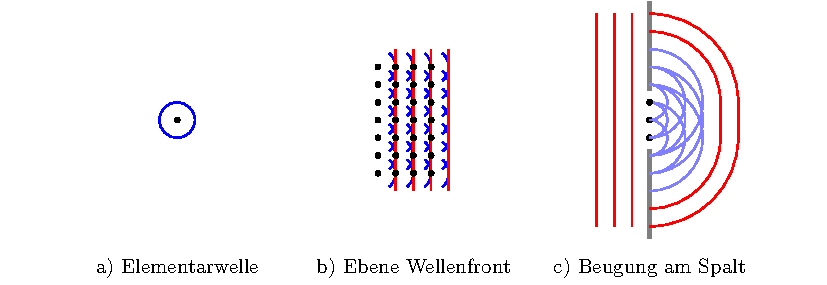
\includegraphics[width=120mm]{papers/opt/images/huygens.pdf}
    \caption{Gemäss dem Prinzip von Huygens kann eine Wellenfront als Überlagerung unendlich vieler Elementarwellen aufgefasst werden.
    Wenn diese Wellenfront auf ein Hindernis trifft, entsteht dahinter eine neue, gebogene Wellenfront.}
    \label{opt:fig:huygens}
\end{figure}


%%%%%%%%%%%%%%%%%%%%%%%%%%%%%%%%%%%%%%%%%%%%%%%%%%%%%%%%%%%%%%%%%%%%%%%%%%%%%%%%%%%%%%%%%%%%%%%%%%%%%%%%%%%%%%%%%%%%%%%%
\subsection{Allgemeines Beugungsintegral}

\begin{figure}
    \centering
    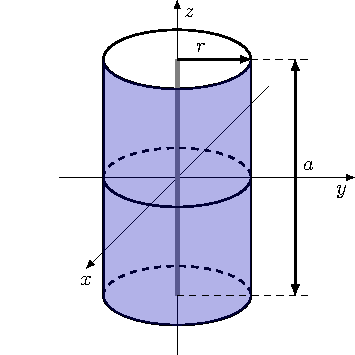
\includegraphics[width=57.34mm]{papers/opt/images/maxwell.pdf}
    \caption{Grau eingefärbt entlang der $z$-Achse ist die Linienquelle dargestellt, welche vom Zylinder mit dem Radius $r$ und der Länge $a$ umschlossen wird.
    Das elektrische Feld $\vec{E}$ breitet sich immer radial und rechtwinklig zur Lichtquelle aus.}
    \label{opt:fig:maxwell}
\end{figure}

Betrachten wir zuerst, wie in Abbildung \ref{opt:fig:maxwell} gezeigt, eine linienförmige Lichtquelle, welche sich axial in positive und negative $z$-Richtung unendlich weit erstreckt.
Verallgemeinert kann es sich bei dieser Art von Quelle um eine beliebige elektromagnetische Quelle handeln.
Somit kann durch Anwenden der ersten Maxwellschen Gleichung
\begin{equation*}
\oint_{S=\partial V} \varepsilon\vec{E} \cdot\, d\vec{S}
=
\int_{V}\rho\, dV
\end{equation*}
die elektrische Feldstärke $\vec{E}$ an jedem beliebigen Punkt in Abhängigkeit vom radialen Abstand $r$ berechnet werden.
Dabei ist $\varepsilon$ die Permittivität, $\rho$ die Ladungsdichte und $V$ das Volumen über dessen Oberfläche $S$ integriert werden muss.
Angewendet auf die gegebene Geometrie des Zylindermantels, lässt sich diese Gleichung mittels $\vec{dS} = r\, d\varphi\, dl \cdot \hat{r}$ und $\vec{E} = E \cdot \hat{r}$ als
\begin{align*}
\int_{0}^{a}\int_{0}^{2\pi} \varepsilon E\cdot \hat{r} \cdot \hat{r} \cdot r\, d\varphi\, dl
&=
Q
\\
\int_{0}^{a}\int_{0}^{2\pi} \varepsilon E\cdot 1 \cdot r\, d\varphi\, dl
&=
Q
\\
2\pi ra\varepsilon E
&=
Q
\end{align*}
schreiben.
Die durch die Deckflächen entstehenden Randeffekte des elektrischen Feldes können aufgrund der infiniten Länge des Zylinders vernachlässigt werden.
Des Weiteren beschreibt $Q$ die durch den Zylindermantel eingeschlossene Ladung.
Zu beachten ist zudem, dass die normierten vektoriellen Grössen $\hat{E} = \hat{r}$ und $\hat{S} = \hat{r}$ parallel verlaufen und sich ihr Skalarprodukt dementsprechend zu 1 vereinfacht.
In anderen Worten, das elektrische Feld $E$ durchtritt die Mantelfläche des Zylinders immer im rechten Winkel.
Nach der elektrischen Feldstärke umgeformt lautet die Gleichung
\begin{equation}
E(r)
=
\frac{Q}{2\pi\varepsilon a} \cdot \frac{1}{r}
=
\vartheta \cdot \frac{1}{r}
,
\label{opt:equation:electric_field}
\end{equation}
wobei der konstante Anteil als $\vartheta$ zusammengefasst wurde.

\begin{figure}
    \centering
    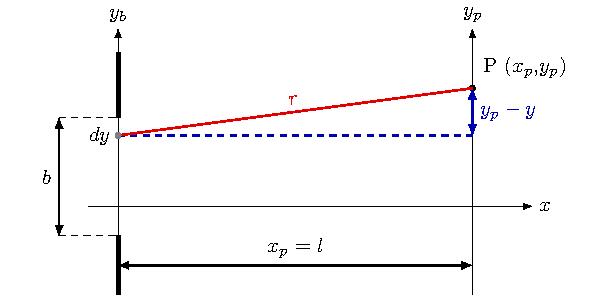
\includegraphics[width=100mm]{papers/opt/images/derivation.pdf}
    \caption{Beugung am Spalt: Die ebene Welle kommt von links her an den Spalt. 
    Von allen $dy$ geht eine Elementarwelle gemäss Abschnitt \ref{opt:subsection:huygens} aus, welche sich am Auswertepunkt $P$ aufsummiert.}
    \label{opt:fig:geometricalShape}
\end{figure}

Angenommen eine planare elektromagnetische Welle, wie in Abbildung \ref{opt:fig:geometricalShape} ersichtlich, treffe nun auf eine Blende mit einer unendlich langen und $b$ breiten Öffnung.
Ganz allgemein lässt sich jede Welle als
\begin{equation}
\zeta(x, t)
=
\zeta_0 \cdot e^{j(\omega t - \vec{k}\cdot\vec{x})}
\label{opt:equation:wave}
\end{equation}
ausdrücken.
Wie in Abschnitt \ref{opt:subsection:huygens} gezeigt, wird diese Welle an der Blende gebeugt.
In Abhängigkeit von der Öffnungsbreite $b$ breitet sich die Welle anschliessend annähernd kreisförmig als neue Wellenfront weiter aus.
Dieses Verhalten der kreisförmigen Ausbreitung kann mittels der zuvor betrachteten Linienquellen modelliert werden.
Unendlich viele dieser Linienquellen sind nun nebeneinander entlang der Öffnungsbreite $b$ angereiht.
Die Auswirkung dieser Quellen kann nun an jedem beliebigen Punkt hinter der Blende durch Superposition der einzelnen Quelleneinflüsse berechnet werden.

Ein Schirm werde nun im Abstand $l$ hinter der Blende angebracht, an welchem die elektrische Feldstärke auf verschiedenen Höhen $y_p$ gemessen werden soll.
Aus der geometrischen Anordnung in Abbildung \ref{opt:fig:geometricalShape} geht hervor, dass
\begin{equation}
r
=
\sqrt{l^2 + (y_p-y)^2}
=
l \sqrt{1 + \frac{(y_p-y)^2}{l^2}}
\label{opt:equation:distance_r}
\end{equation}
beträgt. All diese kleinen Einflüsse $dE$ der Linienquellen mit Breite $dy$ superponieren sich zur gesamten elektrischen Feldstärke am Auswertungspunkt.
Ein solcher Einfluss lässt sich nun mittels der Gleichungen \eqref{opt:equation:electric_field} und \eqref{opt:equation:wave} als
\begin{equation*}
dE
=
E(r) \cdot \zeta(r, t) \cdot dy
=
\frac{\vartheta}{r} \cdot \zeta_0 \cdot e^{j(\omega t - \vec{k}\cdot\vec{r})} \cdot dy
\end{equation*}
beschreiben.
Werden die Einflüsse der Linienquellen über den Spalt integriert, ergibt sich der Ausdruck
\begin{equation*}
E(y_p, t)
=
\int_{y_b}^{y_b+b}\frac{\vartheta\zeta_0}{r} \cdot e^{j(\omega t - \vec{k}\cdot\vec{r})} \,dy
=
\vartheta\zeta_0 \cdot \int_{y_b}^{y_b+b}\frac{e^{j(\omega t - \vec{k}\cdot\vec{r})}}{r} \,dy
.
\end{equation*}
Die Beugung einer Welle an einer beliebigen Blende statt nur an einem Spalt kann mit der Blendenfunktion $f(y)$ als Integral dargestellt werden.
Zu beachten ist, dass diese Funktion nicht nur die Extremwerte 0 und 1, sondern auch jegliche Werte dazwischen annehmen kann.
Dies würde einer teilweise transparenten Blende entsprechen.
Ein Wert von 0 bedeutet dabei, dass kein Licht durchgelassen wird und ein Wert von 1, dass alles Licht die Blende durchdringen kann.
Somit folgt als allgemeinste Form
\begin{align}
E(y_p, t)
=
\vartheta\zeta_0 \cdot \int_{-\infty}^{\infty}f(y)\cdot\frac{e^{j(\omega t - \vec{k}\cdot\vec{r})}}{r} \,dy
.
\label{opt:equation:integral_general}
\end{align}
Dieses Integral ist für jeden Auswertungspunkt allgemein gültig.
Wie sich aber zeigen wird, ist dieses Integral, genauer gesagt $r$ aus Gleichung \eqref{opt:equation:distance_r}, nicht fundamental genug, um es analytisch lösen zu können.
Die folgenden Approximationen von $r$ sollen dabei diese Hürde umgehen.


%%%%%%%%%%%%%%%%%%%%%%%%%%%%%%%%%%%%%%%%%%%%%%%%%%%%%%%%%%%%%%%%%%%%%%%%%%%%%%%%%%%%%%%%%%%%%%%%%%%%%%%%%%%%%%%%%%%%%%%%
\subsection{Fresnel-Approximation}
\label{opt:sec:fresnel}
In einer ersten Vereinfachung wird das allgemeine Beugungsintegral aus \eqref{opt:equation:integral_general} für kleine Winkel approximiert.
Für weitere Schritte ist die Bedingung
\begin{equation}
y, y_p
\ll
l
\label{opt:equation:condition_fresnel}
\end{equation}
nötig.
Durch Anwenden der Binominalexpansion
\begin{equation*}
(1 + \varepsilon)^n
\approx
1 + n\varepsilon
,
\end{equation*}
unter der Voraussetzung, dass $\varepsilon \ll 1$ gilt, ist es möglich den Wurzelausdruck aus Gleichung \eqref{opt:equation:distance_r} noch weiter zu vereinfachen.
Mit Hilfe der Vorbedingungen aus Gleichung \eqref{opt:equation:condition_fresnel} ist
\begin{equation*}
(y_p-y)^2
\ll
l^2
\end{equation*}
gegeben.
Somit kann die Bedingung für
\begin{equation*}
\varepsilon
=
\frac{(y_p-y)^2}{l^2}
\ll
1
\end{equation*}
eingehalten werden.
Gleichung \eqref{opt:equation:distance_r} vereinfacht sich demnach näherungsweise zu
\begin{equation}
r
=
l \sqrt{1 + \frac{(y_p-y)^2}{l^2}}
\approx
l \left(1 - \frac{(y_p-y)^2}{2l^2}\right)
=
l - \frac{(y_p-y)^2}{2l}
.
\label{opt:equation:distance_r_fresnel}
\end{equation}
Durch Ausklammern von Konstanten und Einsetzen der Gleichung \eqref{opt:equation:distance_r_fresnel} vereinfacht sich das Integral aus Gleichung \eqref{opt:equation:integral_general} weiter zu
\begin{align*}
E(y_p, t)
&=
\vartheta\zeta_0 \cdot e^{j\omega t} \cdot \int_{-\infty}^{\infty}f(y)\cdot\frac{e^{-j\vec{k}\cdot\vec{r}}}{r} \,dy
\\
&=
\vartheta\zeta_0 \cdot e^{j\omega t} \cdot \int_{-\infty}^{\infty}f(y)\cdot\frac{e^{-jkr}}{r} \,dy
\\
&\approx
\vartheta\zeta_0 \cdot e^{j\omega t} \cdot \int_{-\infty}^{\infty}f(y)\cdot\frac{e^{-jkl} \cdot e^{jk\frac{(y_p-y)^2}{2l}}}{l - \frac{(y_p-y)^2}{2l}} \,dy
\\
&=
\vartheta\zeta_0 \cdot e^{j\omega t} \cdot e^{-jkl} \cdot \int_{-\infty}^{\infty}f(y)\cdot\frac{e^{jk\frac{(y_p-y)^2}{2l}}}{l - \frac{(y_p-y)^2}{2l}} \,dy
.
\end{align*}
Wiederum konnte das Skalarprodukt der normierten Grössen $\hat{k}$ und $\hat{r}$ aufgrund Parallelität als 1 gekürzt geschrieben werden.
Des Weiteren kann der Ausdruck 
\begin{equation*}
    l - \frac{(y_p-y)^2}{2l}
\end{equation*}
im Nenner des Integrals als $l$ vereinfacht werden.
Zulässig ist dies nur, weil $y_p, y \ll l$ erfüllt ist.
Dasselbe Prinzip darf jedoch nicht auf den Exponenten angewandt werden, da dieser mit dem Faktor der Wellenzahl multipliziert wird und der Term
\begin{equation*}
    k \frac{(y_p-y)^2}{2l}
\end{equation*}
somit nicht vernachlässigbar klein wird.
Der Zeitpunkt der Auswertung ist nicht von Interesse, da dieser lediglich die Phase der Welle beeinflusst.
Mittels $t = 0$ vereinfacht sich der Ausdruck zu
\begin{align}
E(y_p, t = 0)
&=
\vartheta\zeta_0 \cdot e^{j\omega t} \cdot e^{-jkl} \cdot \int_{-\infty}^{\infty}f(y)\cdot\frac{e^{jk\frac{(y_p-y)^2}{2l}}}{l} \,dy
\notag
\\
&=
\frac{\vartheta\zeta_0}{l} \cdot 1 \cdot e^{-jkl} \cdot \int_{-\infty}^{\infty}f(y)\cdot e^{jk\frac{(y_p-y)^2}{2l}} \,dy
\notag
\\
&=
\frac{\vartheta\zeta_0}{l} \cdot e^{-jkl} \cdot \int_{-\infty}^{\infty}f(y)\cdot e^{jk\frac{(y_p^2 - 2y_py + y^2)}{2l}} \,dy
.
\label{opt:equation:integral_fresnel}
\end{align}
Das hiermit erhaltene Integral wird auch als das Fresnel-Beugungsintegral\footnote{Benannt nach dem französischen Physiker Augustin Fresnel; daher ausgesprochen mit einem stummen \emph{s}.}
bezeichnet und entspricht einer Nahfeldnäherung.
Anders als von der Bezeichnung zu erwarten wäre, darf diese Näherung nicht direkt hinter der Blende angewendet werden.
Die Voraussetzung $y, y_p \ll l$ aus Gleichung \eqref{opt:equation:condition_fresnel} muss erfüllt sein.
Ansonsten muss das allgemeine Beugungsintegral für die Berechnung verwendet werden.

\subsection{Fraunhofer-Approximation}
\label{opt:sec:fraunhofer}
Die Fresnel-Approximation aus \eqref{opt:equation:integral_fresnel} kann mittels der Fraunhofer-Approximation\footnote{Benannt nach dem deutschen Physiker Joseph Fraunhofer.} weiter vereinfacht werden.
Dafür wird die Distanz zwischen der Blende und der Auswertungsebene noch weiter erhöht.
Damit wird es möglich, das Integral in Bezug auf die Distanz $y$ zwischen der Quelle und der Auswertungsebene zu linearisieren.
Ist nun
\begin{equation*}
y
\ll
y_p
\ll
l
\end{equation*}
gegeben, kann der Ausdruck $y_p^2 - 2y_py + y^2$ aus Gleichung \eqref{opt:equation:integral_fresnel} weiter approximiert werden.
Unter Berücksichtigung dieser Bedingung ist $y^2 \ll 2y_py$, wodurch der Term $y^2$ vernachlässigt werden kann.
Daraus folgt
\begin{align}
E(y_p)
&\approx
\frac{\vartheta\zeta_0}{l} \cdot e^{-jkl} \cdot \int_{-\infty}^{\infty}f(y)\cdot e^{jk\frac{(y_p^2 - 2y_py)}{2l}} \,dy
\notag
\\
&=
\frac{\vartheta\zeta_0}{l} \cdot e^{-jkl} \cdot e^{jk\frac{y_p^2}{2l}} \cdot \int_{-\infty}^{\infty}f(y)\cdot e^{-jk\frac{y_py}{l}} \,dy
\notag
\\
&=
\frac{\vartheta\zeta_0}{l} \cdot e^{-jk\left(l-\frac{y_p^2}{2l}\right)} \cdot \int_{-\infty}^{\infty}f(y)\cdot e^{-j\frac{ky_p}{l}y} \,dy
.
\label{opt:equation:integral_fraunhofer}
\end{align}
Mit Hilfe der Fresnel-Approximation und anschliessend der Fraunhofer-Approximation 
konnte das allgemeingültige Beugungsintegral auf eine analytisch einfach lösbare Form gebracht werden.
Das somit entstandene Integral entspricht bis auf einige Vorfaktoren gerade der Fourier-Transformation der Blendenfunktion $f(y)$.

Gleichung \eqref{opt:equation:integral_fraunhofer} ist dementsprechend bereits das zentrale Ergebnis dieses Papers.
In einem weiteren Schritt könnte das Resultat so erweitert werden, dass die Blendenfunktion auf eine Funktion mehrere Variablen $f(y,z)$ in $y$ und $z$-Richtung zu liegen kommt.
Auf diesen zusätzlichen Schritt wird in diesem Paper aber nicht weiter eingegangen.
